\subsection{重回帰分析について}
重回帰分析に使用したデータは\ref{tab:regression-data}に示す。
このデータを用いて、身長・胸囲から体重を予測する重回帰分析を行った。
身長を$h$、胸囲を$c$、体重を$w$として、各ベクトル量$\bm{h}=\trans{[h_1, h_2, \dots]}$などと定義する。
このとき、
\begin{equation}\label{eq:regression-solve-equation}
	\bm{w} = \begin{bmatrix} \bm{1} & \bm{h} & \bm{c} \end{bmatrix} \bm{b}
\end{equation}
として、最小二乗法により$\bm{b}$を求めることで、重回帰分析を行った。\footnote{
	$\begin{bmatrix} \bm{1} & \bm{h} & \bm{c} \end{bmatrix}$の部分に関してであるが、
	これは、次のように各ベクトル量を並べた行列である。
	\begin{equation*}
		\begin{bmatrix} 1 & h_1 & c_1 \\ 1 & h_2 & c_2 \\ \vdots & \vdots & \vdots \end{bmatrix}
	\end{equation*}
}
$\bm{b}$は3次元ベクトルである。

\ref{eq:normal-equation-multiple}式より、\ref{eq:regression-solve-equation}式の解$\bm{\hat{b}}$は、
$X=\begin{bmatrix}\bm{1} & \bm{h} & \bm{c}\end{bmatrix}$として、
\begin{equation}
	\bm{\hat{b}} = \left( \trans{X}X \right)^{-1} \trans{X} \bm{w}
\end{equation}
であり、コンピュータで計算した結果、
\begin{equation}\label{eq:regression-result}
	\bm{\hat{b}} = \begin{pmatrix}
		-82.7519 \\
		0.3462   \\
		0.9584
	\end{pmatrix}
\end{equation}
と得られた。

この解の妥当性を評価する。
実際に得られた値$\bm{w}$と、予測値$\bm{\hat{w}}$の関係を図\ref{fig:regression-ex-graph}に示す。
\footnote{
	図中の$y$と$\bm{w}$、$\hat{y}$と$\bm{\hat{w}}$は同じものである。
}
図を見ると、概ね右上がりの直線上、すなわち$y=\hat{y}$の直線の近くに点が分布していることがわかる。
\begin{figure}
	\centering
	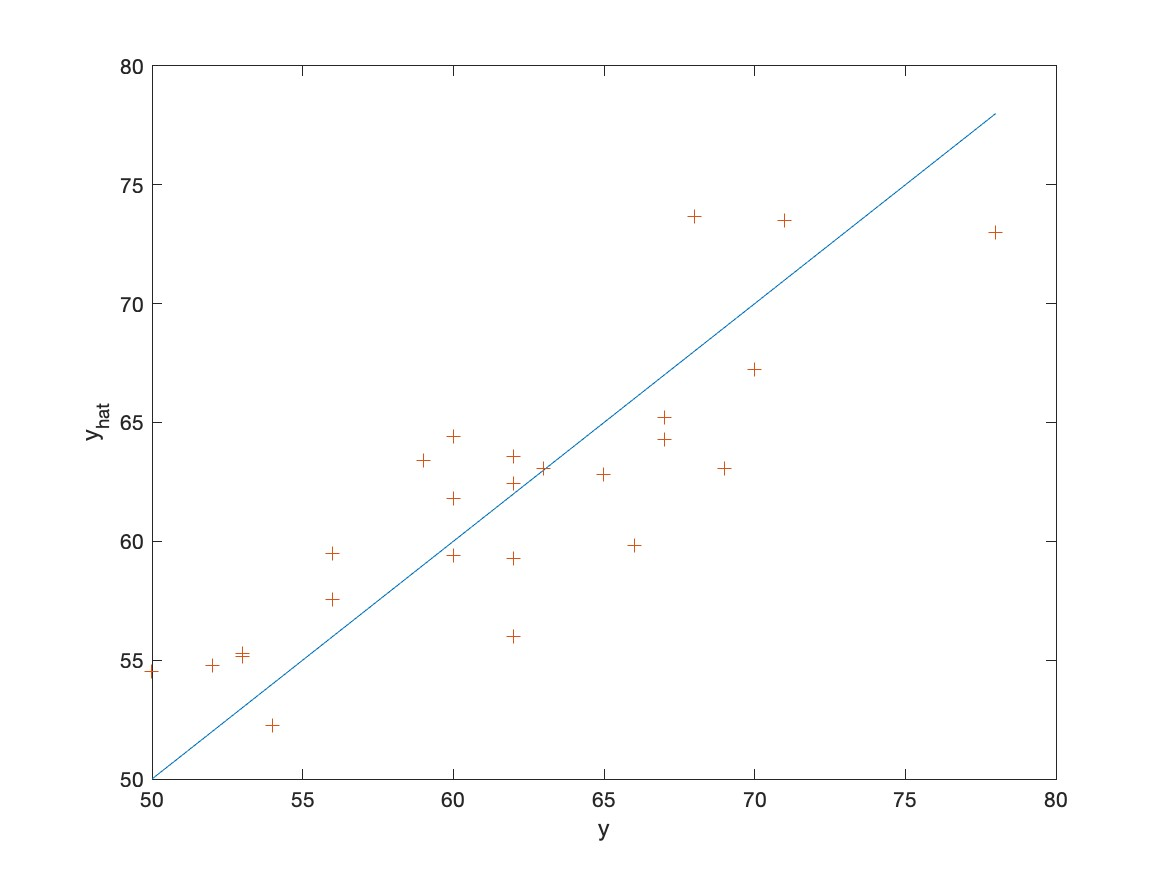
\includegraphics[width=0.8\linewidth]{src/figures/regression/regression_ex_graph.jpg}
	\caption{実際の値$y$と予測値$\hat{y}$の関係}\label{fig:regression-ex-graph}
\end{figure}

さらに、\ref{eq:regression-mean}式から、$\bm{w}$と$\bm{\hat{w}}$の平均値を比較するとともに$61.8000$となり一致する。
また、\ref{eq:coefficent-determination}式より重相関係数を計算すると、$R=0.8538$となった。
1に近い値であり、この重回帰分析は有効であるといえる。
